\section{The spectrum of $\tilde{\boldsymbol{\Delta}}_{\text{sym}}$}

The normalized Laplacian defined on graphs with self-loops, $\tilde{\boldsymbol{\Delta}}_{\text{sym}}$, consists of an instance of generalized graph Laplacians and hold the interpretation as a difference operator, i.e. for any signal $\rvx \in \mathbb{R}^n$ it satisfies 
\begin{equation}
(\tilde{\boldsymbol{\Delta}}_{\text{sym}} \rvx)_i = \sum_{j} \frac{\tilde{a}_{ij}}{\sqrt{d_i + \gamma}} \left(\frac{x_i}{\sqrt{d_i + \gamma}} - \frac{x_j}{\sqrt{d_j + \gamma}}\right). \nonumber
\end{equation}

Here, we prove several properties regarding its spectrum.

\begin{lemma}
(Non-negativity of $\tilde{\boldsymbol{\Delta}}_{\text{sym}}$) The augmented normalized Laplacian matrix is symmetric positive semi-definite.
\end{lemma}
\begin{proof}

The quadratic form associated with $\tilde{\boldsymbol{\Delta}}_{\text{sym}}$ is
\begin{align}
    & \rvx^\top\tilde{\boldsymbol{\Delta}}_{\text{sym}}\rvx  = \sum_i x_i^2 - \sum_i \sum_j\frac{\tilde{a}_{ij} x_i x_j}{\sqrt{(d_i + \gamma)(d_j + \gamma)}} \nonumber \\
    & = \frac{1}{2} \left( \sum_i x_i^2 + \sum_j x_j^2  - \sum_i \sum_j \frac{2\tilde{a}_{ij} x_i x_j}{\sqrt{(d_i + \gamma)(d_j + \gamma)}}\right) \nonumber \\
    & = \frac{1}{2} \left(\sum_i \sum_j \frac{\tilde{a}_{ij} x_i^2}{d_i + \gamma} + \sum_j \sum_i \frac{\tilde{a}_{ij} x_j^2}{d_j + \gamma} \right.
     \nonumber \\ & \left. \quad \quad - \sum_i \sum_j  \frac{2\tilde{a}_{ij} x_i x_j}{\sqrt{(d_i + \gamma)(d_j + \gamma)}}\right) \nonumber \\
    &  = \frac{1}{2} \sum_i \sum_j \tilde{a}_{ij}\left(\frac{x_i}{\sqrt{d_i + \gamma}} - \frac{x_j}{\sqrt{d_j + \gamma}}\right)^2 \geq 0 \label{eq:norm_laplacian_self_loops}
\end{align}


\end{proof}

\begin{lemma}
\label{lem:0_eig}
$0$ is an eigenvalue of both $\boldsymbol{\Delta}_{\text{sym}}$ and $\tilde{\boldsymbol{\Delta}}_{\text{sym}}$.
\end{lemma}
\begin{proof}
First, note that $\rvv=[1,\ldots,1]^\top$ is an eigenvector of $\boldsymbol{\Delta}$ associated with eigenvalue $0$, i.e., $\boldsymbol{\Delta} \rvv = (\rmD-\rmA)\rvv = \mathbf{0}$.

Also, we have that $\tilde{\boldsymbol{\Delta}}_{\text{sym}} = \tilde{\rmD}^{-1/2}(\tilde{\rmD} - \tilde{\rmA})\tilde{\rmD}^{-1/2} = \tilde{\rmD}^{-1/2}\boldsymbol{\Delta}\tilde{\rmD}^{-1/2}$. Denote $\rvv_1=\tilde{\rmD}^{1/2}\rvv$, then
$$
\tilde{\boldsymbol{\Delta}}_{\text{sym}}\rvv_1 = \tilde{\rmD}^{-1/2}\boldsymbol{\Delta}\tilde{\rmD}^{-1/2}\tilde{\rmD}^{1/2}\rvv = \tilde{\rmD}^{-1/2} \boldsymbol{\Delta} \rvv = \mathbf{0}.
$$

Therefore, $\rvv_1=\tilde{\rmD}^{1/2}\rvv$ is an eigenvector of $\tilde{\boldsymbol{\Delta}}_{\text{sym}}$ associated with eigenvalue $0$, which is then the smallest eigenvalue from the non-negativity of $\tilde{\boldsymbol{\Delta}}_{\text{sym}}$. Likewise, 0 can be proved to be the smallest eigenvalues of $\boldsymbol{\Delta}_{\text{sym}}$.
\end{proof}

\begin{lemma}
\label{lem:adj_eig}
Let $\beta_1 \leq \beta_2 \leq \dots \leq \beta_n$ denote eigenvalues of $\rmD^{-1/2}\rmA \rmD^{-1/2}$ and $\alpha_1 \leq \alpha_2 \leq \dots \leq \alpha_n$ be the eigenvalues of $\tilde{\rmD}^{-1/2}\rmA\tilde{\rmD}^{-1/2}$. Then,
\begin{align} \label{eq:bounds_norm_adj}
    & \alpha_1 \geq \frac{\max_i d_i}{\gamma+\max_i d_i}\beta_1, &\alpha_n \leq \frac{\min_i{d_i}}{\gamma + \min_i{d_i}}.
\end{align}
\end{lemma}

\begin{proof}

We have shown that 0 is an eigenvalue of $\boldsymbol{\Delta}_{\text{sym}}$. Since $\rmD^{-1/2}\rmA \rmD^{-1/2} = \rmI - \boldsymbol{\Delta}_{\text{sym}}$, then $1$ is an eigenvalue of $\rmD^{-1/2}\rmA \rmD^{-1/2}$. More specifically, $\beta_n = 1$. In addition, by combining the fact that $\Tr(\rmD^{-1/2}\rmA\rmD^{-1/2})=0=\sum_i \beta_i$ with $\beta_n = 1$, we conclude that $\beta_1 < 0$.

By choosing $\rvx$ such that $\lVert \rvx \rVert =1$ and $\rvy=\rmD^{1/2}\tilde{\rmD}^{-1/2} \rvx$, we have that $\|\rvy\|^2=\sum\limits_i\frac{d_i}{d_i+\gamma}x_i^2$ and $\frac{\min_i d_i}{\gamma+\min_i d_i}\leq \|\rvy\|^2\leq \frac{\max_i d_i}{\gamma+\max_i d_i}$. Hence, we use the Rayleigh quotient to provide a lower bound to $\alpha_1$:
\begin{align*}
\alpha_1 & = \min_{\|\rvx\|=1} \left(\rvx^\top\tilde{\rmD}^{-1/2} \rmA \tilde{\rmD}^{-1/2} \rvx \right) \\
& = \min_{\|\rvx\|=1} \left( \rvy^\top\rmD^{-1/2} \rmA \rmD^{-1/2} \rvy \right) \text{(by replacing variable)} \\
&= \min_{\|\rvx\|=1} \left( \frac{\rvy^\top\rmD^{-1/2} \rmA \rmD^{-1/2}\rvy}{\|\rvy\|^2}\|\rvy\|^2 \right) \\
&\geq \min_{\|\rvx\|=1} \left( \frac{\rvy^\top\rmD^{-1/2} \rmA \rmD^{-1/2} \rvy}{\|\rvy\|^2} \right) \max_{\|\rvx\|=1} \left( \|\rvy\|^2 \right) \\
& ( \because  \min (AB) \geq \min (A) \max(B) \text{ if } \min (A) < 0, \forall B > 0,
\\
&\text{ and \quad} 
\min_{\|\rvx\|=1} \left( \frac{\rvy^\top\rmD^{-1/2} \rmA \rmD^{-1/2} \rvy}{\|\rvy\|^2} \right) = \beta_1 < 0 ) \\
&= \beta_1\max_{\|\rvx\|=1} \|\rvy\|^2 \\
&\geq \frac{\max_i d_i}{\gamma+\max_i d_i}\beta_1.\\
 \end{align*}

One may employ similar steps to prove the second inequality in \autoref{eq:bounds_norm_adj}.

\end{proof}

\begin{proof} [Proof of Theorem 1] 
Note that $\tilde{\boldsymbol{\Delta}}_{\text{sym}} = \rmI - \gamma \tilde{\rmD}^{-1} - \tilde{\rmD}^{-1/2}\rmA\tilde{\rmD}^{-1/2}$. Using the results in Lemma \autoref{lem:adj_eig}, we show that the largest eigenvalue $\tilde{\lambda}_n$ of $\tilde{\boldsymbol{\Delta}}_{\text{sym}}$ is
\begin{align} \label{eq:bound_laplacians}
        \tilde{\lambda}_n  & = \max_{\|\rvx\|=1} \rvx^\top(\rmI - \gamma \tilde{\rmD}^{-1} - \tilde{\rmD}^{-1/2}\rmA\tilde{\rmD}^{-1/2})\rvx  \nonumber \\
               & \leq  1 - \min_{\|\rvx\|=1} \gamma \rvx^\top \tilde{\rmD}^{-1} \rvx - \min_{\|\rvx\|=1} \rvx^\top \tilde{\rmD}^{-1/2} \rmA \tilde{\rmD}^{-1/2} \rvx \nonumber \\
               & = 1 - \frac{\gamma}{\gamma + \max_{i} d_i} - \alpha_1 \nonumber \\
               & \leq  1 - \frac{\gamma}{\gamma + \max_{i} d_i} - \frac{\max_i d_i}{\gamma + \max_i d_i} \beta_1 \nonumber \\
               & <  1 - \frac{\max_i d_i}{\gamma + \max_i d_i} \beta_1 \quad (\gamma > 0 \text{ and } \beta_1 < 0) \nonumber \\
               & < 1 - \beta_1 = \lambda_n
\end{align}


\end{proof}

\section{Experiment Details}
\label{sec:exp-details}
\paragraph{Node Classification.}
We empirically find that on Reddit dataset for \method{}, it is crucial to normalize the features into zero mean and univariate. 

\paragraph{Training Time Benchmarking.} We hereby describe the experiment setup of Figure 3.
\citet{FastGCN} benchmark the training time of FastGCN on CPU, and as a result, it is difficult to compare numerical values across reports.
Moreover, we found the performance of FastGCN improved with a smaller early stopping window (10 epochs); therefore, we could decrease the model's training time.
We provide the data underpinning Figure 3 in \autoref{table:citation-time} and \autoref{table:reddit-time}.
%
\begin{table}[htb!]
\centering
        \small
        \caption{Training time (seconds) of graph neural networks on Citation Networks. Numbers are averaged over 10 runs.}
        \label{table:citation-time}
        \begin{tabular}{l|c|c|c}
        \toprule
        Models & Cora & Citeseer & Pubmed \\ 
        \midrule
        % \midrule
        GCN & $0.49$ & $0.59$ & $8.31$ \\
        % GCN - test w/o relu & $81.8 \pm{0.66}$ & $70.7\pm 0.93$ & $79.1 \pm{0.65}$ \\
        GAT & $63.10$ & $118.10$ &  $121.74$ \\
        FastGCN & $2.47$ & $3.96 $ & $1.77$ \\
        GIN & $2.09$ &  $4.47$ & $26.15$ \\
        LNet & $15.02$ & $49.16$  & $266.47$ \\
        AdaLNet & $10.15$ & $31.80$ & $222.21$ \\
        DGI & $21.24$ & $21.06$ & $76.20$\\
        {\color{modelblue} \method{}} & $0.13$ & $0.14$ & $0.29$ \\
         \bottomrule
        \end{tabular}
\end{table}
%
\begin{table}[htb!]
        \centering
        \small
        \caption{Training time (seconds) on Reddit dataset.}
        \label{table:reddit-time}
        \begin{tabular}{l|l}
        \toprule
        Model & Time(s) $\downarrow$ \\
         \midrule
        SAGE-mean & $78.54$\\
        SAGE-LSTM & $486.53$\\
        SAGE-GCN & $86.86$\\
        FastGCN & $270.45$\\
        {\color{modelblue} \method{}} & $2.70$ \\
        \bottomrule
        \end{tabular}
\end{table}
\begin{figure*}[htb] 
\centering
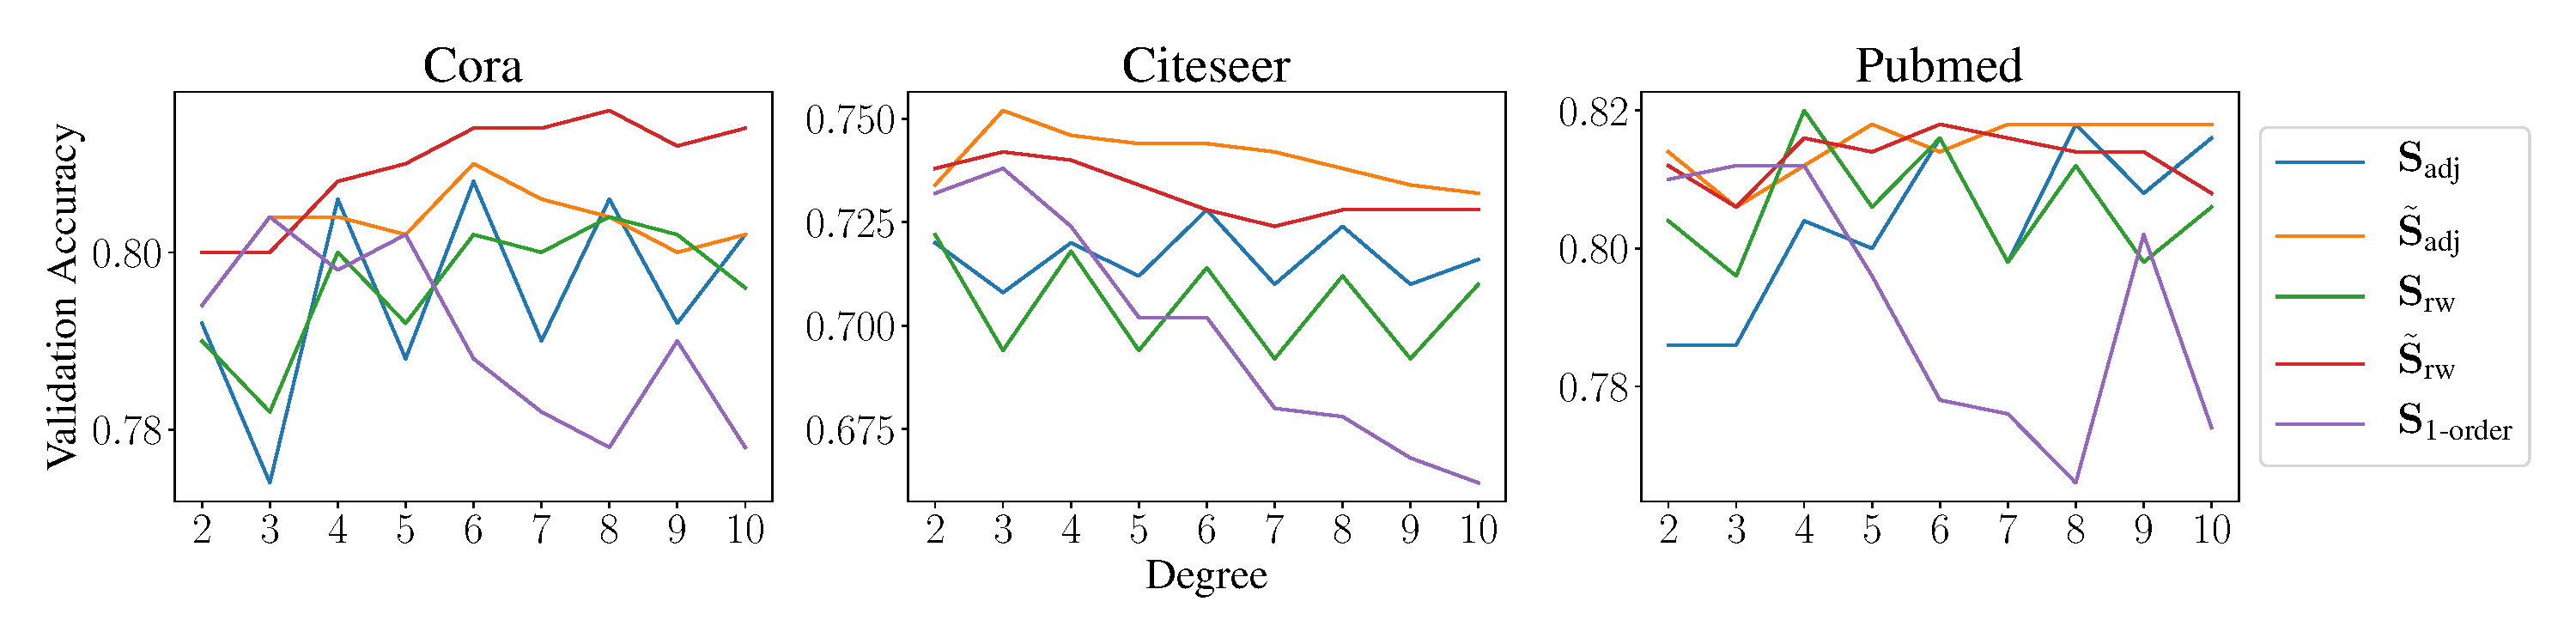
\includegraphics[width=0.9\textwidth]{figures/propagation.pdf}
\caption{Validation accuracy with \method{} using different propagation matrices.}
\label{fig:propagation-ablation}
\end{figure*}
%
\paragraph{Text Classification.} 
\citet{textGCN} use one-hot features for the word and document nodes. In training SGC, we normalize the features to be between 0 and 1 \textbf{after propagation} and train with L-BFGS for 3 steps. We tune the only hyperparameter, weight decay, using hyperopt\cite{hyperopt} for 60 iterations. Note that we cannot apply this feature normalization for TextGCN because the propagation cannot be precomputed. 
%
\paragraph{Semi-supervised User Geolocation.}
We replace the 4-layer, highway-connection GCN with a 3rd degree propagation matrix ($K=3$) SGC and use the same set of hyperparameters as \citet{Rahimi18}. All experiments on the GEOTEXT dataset are conducted on a single Nvidia GTX-1080Ti GPU while the ones on the TWITTER-NA and TWITTER-WORLD datasets are excuded with 10 cores of the Intel(R) Xeon(R) Silver 4114 CPU (2.20GHz). Instead of collapsing all linear transformations, we keep two of them which we find performing slightly better possibly due to . Despite of this subtle variation, the model is still linear.
%
\paragraph{Relation Extraction.}
We replace the 2-layer GCN with a 2nd degree propagation matrix ($K=2$) SGC and remove the intermediate dropout. We keep other hyperparameters unchanged, including learning rate and regularization. Similar to \citet{relation-extraction}, we report the best validation accuracy with early stopping.
%
\paragraph{Zero-shot Image Classification.}
We replace the 6-layer GCN (hidden size: 2048, 2048, 1024, 1024, 512, 2048) baseline with an 6-layer MLP (hidden size: 512, 512, 512, 1024, 1024, 2048) followed by a SGC with $K=6$. Following \cite{wang2018zero}, we only apply dropout to the output of SGC. Due to the slow evaluation of this task, we do not tune the dropout rate or other hyperparameters. Rather, we follow the GCNZ code and use learning rate of 0.001, weight decay of 0.0005, and dropout rate of 0.5. We also train the models with ADAM~\cite{adam} for 300 epochs.

\section{Additional Experiments}
%
%
\paragraph{Random Splits for Citation Networks.}
Possibly due to their limited size, the citation networks are known to be unstable. 
Accordingly, we conduct an additional 10 experiments on random splits of the training set while maintaining the same validation and test sets. 
%
\begin{table}[th!]
\small
\centering
\caption{Test accuracy (\%) on citation networks (random splits). $^\dagger$We remove the outliers (accuracy $< 0.7/0.65/0.75$) when calculating their statistics due to high variance.}
\label{table:citation-random}
\begin{tabular}{l|c|c|c}
\toprule
 & Cora & Citeseer & Pubmed \\ 
\midrule
\multicolumn{4}{l}{\textbf{Ours:}} \\
GCN &  $80.53 \pm{1.40}$ & $70.67\pm{2.90}$ & $77.09 \pm{2.95}$\\
% GCN - test w/o relu  & $80.18 \pm{1.65}$ & $70.98 \pm 2.93$  & $77.14 \pm{2.99}$\\
GIN  & $76.94 \pm 1.24$ & $66.56 \pm 2.27$ & $74.46 \pm 2.19$ \\
LNet & $74.23 \pm 4.50^\dagger$ & $67.26 \pm 0.81^\dagger$ & $77.20 \pm 2.03^\dagger$ \\
AdaLNet & $72.68 \pm 1.45^\dagger$ & $71.04 \pm 0.95^\dagger$ & $77.53 \pm 1.76^\dagger$ \\
GAT  & $82.29 \pm{1.16}$ & $72.6 \pm{0.58}$  & $78.79 \pm{1.41}$ \\
{\color{modelblue} \method{}} & $80.62 \pm{1.21}$ & $71.40 \pm{3.92}$ & $77.02 \pm{1.62} $\\
 \bottomrule
\end{tabular}
\end{table}
%
\paragraph{Propagation choice.}
We conduct an ablation study with different choices of propagation matrix, namely:
\begin{itemize}
\item[] Normalized Adjacency: $\mathbf{S}_{\text{adj}} = \rmD^{-1/2}\rmA \rmD^{-1/2}$
\item[] Random Walk Adjacency $\mathbf{S}_{\text{rw}} = \rmD^{-1}\rmA$
\item[] Aug. Normalized Adjacency $\tilde{\mathbf{S}}_{\text{adj}} = \tilde{\rmD}^{-1/2}\tilde{\rmA} \tilde{\rmD}^{-1/2}$ \item[] Aug. Random Walk $\tilde{\mathbf{S}}_{\text{rw}} = \tilde{\rmD}^{-1} \tilde{\rmA}$ 
\item[] First-Order Cheby $\mathbf{S}_{\text{1-order}}=(\rmI + \rmD^{-1/2}\rmA \rmD^{-1/2} )$
\end{itemize}

We investigate the effect of propagation steps $K \in \{2..10\}$ on validation set accuracy. 
We use hyperopt to tune L2-regularization and leave all other hyperparameters unchanged. \autoref{fig:propagation-ablation} depicts the validation results achieved by varying the degree of different propagation matrices.

We see that augmented propagation matrices (i.e. those with self-loops) attain higher accuracy and more stable performance across various propagation depths. Specifically, the accuracy of $\mathbf{S}_{\text{1-order}}$ tends to deteriorate as the power $K$ increases, and this results suggests using large filter coefficients on low frequencies degrades \method{} performance on semi-supervised tasks.

Another pattern is that odd powers of $K$ cause a significant performance drop for the normalized adjacency and random walk propagation matrices. This demonstrates how odd powers of the un-augmented propagation matrix use negative filter coefficients on high frequency information. Adding self-loops to the propagation matrix shrinks the spectrum such that the largest eigenvalues decrease from $\approx 2$ to $\approx 1.5$ on the citation network datasets. By effectively shrinking the spectrum, the effect of negative filter coefficients on high frequencies is minimized, and as a result, using odd-powers of $K$ does not degrade the performance of augmented propagation matrices. For non-augmented propagation matrices --- where the largest eigenvalue is approximately 2 --- negative coefficients significantly distort the signal, which leads to decreased accuracy. Therefore, adding self-loops constructs a better domain in which fixed filters can operate. 

\begin{table}[h]
    \centering
    \begin{tabular}{c|cc}
    \toprule
    \# Training Samples & \method{} & GCN \\
    \midrule
    1 & 33.16 & 32.94 \\
    5 & 63.74 & 60.68 \\
    10 & 72.04 & 71.46 \\
    20 & 80.30 & 80.16 \\
    40 & 85.56 & 85.38 \\
    80 & 90.08 & 90.44 \\
    \bottomrule
    \end{tabular}
    \caption{Validation Accuracy (\%) when \method{} and GCN are trained with different amounts of data on Cora. The validation accuracy is averaged over 10 random training splits such that each class has the same number of training examples.} 
    \label{tab:data_ablation}
\end{table}

\paragraph{Data amount.}
We also investigated the effect of training dataset size on accuracy. 
As demonstrated in Table~\ref{tab:data_ablation}, \method{} continues to perform similarly to GCN as the training dataset size is reduced, and even outperforms GCN when there are fewer than $5$ training samples. We reason this study demonstrates \method{} has at least the same modeling capacity as GCN.
%
